\begin{proof}
    By contradiction. Let $m = k_1 + k_2 + k_3$ and let $k_1, k_2, k_3$ be
    polynomial functions of $\kappa$. Let $Q$ be a $k$-stable suffix sensitive
    chain predicate. Assume NIPoPoWs on $Q$ is insecure. Then, during an
    execution at some round $r_3$, $Q(\chain)$ is defined and the verifier $V$
    disagrees with all honest miners. Assume the execution is typical. $V$
    communicates with adversary $\mathcal{A}$ and honest prover $B$.  The
    verifier receives proofs $\pi_\mathcal{A}, \pi_B$. Because $B$ is honest,
    $\pi_B$ is a proof constructed based on underlying blockchain $\chain_B$
    (with $\pi_B \subseteq \chain_B$) which $B$ has adopted during round $r_3$
    at which $\pi_B$ was generated. Furthermore, $\pi_\mathcal{A}$ was generated
    at round $r_3' \leq r_3$.

    The verifier outputs $\lnot Q(\chain_B)$, and so
    $\textsf{Verify}^Q_{m,k} = \lnot Q(\chain_B)$. Thus it is necessary that
    $\pi_\mathcal{A} \geq \pi_B$, otherwise, because $Q$
    is suffix sensitive, $\textsf{Verify}^Q$ would have returned $Q(\chain_B)$.
    We now show that $\pi_\mathcal{A} \geq \pi_B$ is a negligible event.

    Let $b = \textsf{LCA}(\pi_\mathcal{A}, \pi_B)$ and let $b^*$ be
    the most recent honestly generated block in $\chain_B$ preceding $b$ (and
    note that $b^*$ necessarily exists because Genesis is honestly generated).
    Let the levels of comparison decided by the verifier be $\mu_\mathcal{A}$
    and $\mu_B$ respectively.
    Let $\mu_B'$ be the adequate level of proof $\pi_B$ with respect to block
    $b$. Call $\alpha_\mathcal{A} =
    \pi_\mathcal{A}\upchain^{\mu_\mathcal{A}}\{b:\}$,
    $\alpha'_B = \pi_B\upchain^{\mu_B'}\{b:\}$.

    We show showing three successive claims: First, $\alpha_\mathcal{A}$ and
    $\alpha'_B\downchain$ are mostly disjoint. Second, $\alpha_\mathcal{A}$
    contains mostly adversarially-generated blocks. And third, the adversary is
    able to produce this $\alpha_\mathcal{A}$ with negligible probability.

    \textbf{Claim 1a: } If $\mu_B' \leq \mu_\mathcal{A}$ then
    $\alpha_\mathcal{A}[1:]$ and $\alpha_B[1:]\downchain$ are completely
    disjoint.

    Applying Lemma~\ref{lem.allblocks}
    to $\chain_B\{b:\}\upchain^{\mu_B'}$ we see that
    $\chain_B\{b:\}\upchain^{\mu_B'} = \pi_B\upchain^{\mu_B'}\{b:\}$ and so
    $\pi_B\upchain^{\mu_B'}\{b:\}[1:] \cap
    \pi_\mathcal{A}\upchain^{\mu_\mathcal{A}}\{b:\}[1:] = \emptyset$.

    \begin{figure*}
        \caption{Two competing proofs at different levels.}
        \centering
        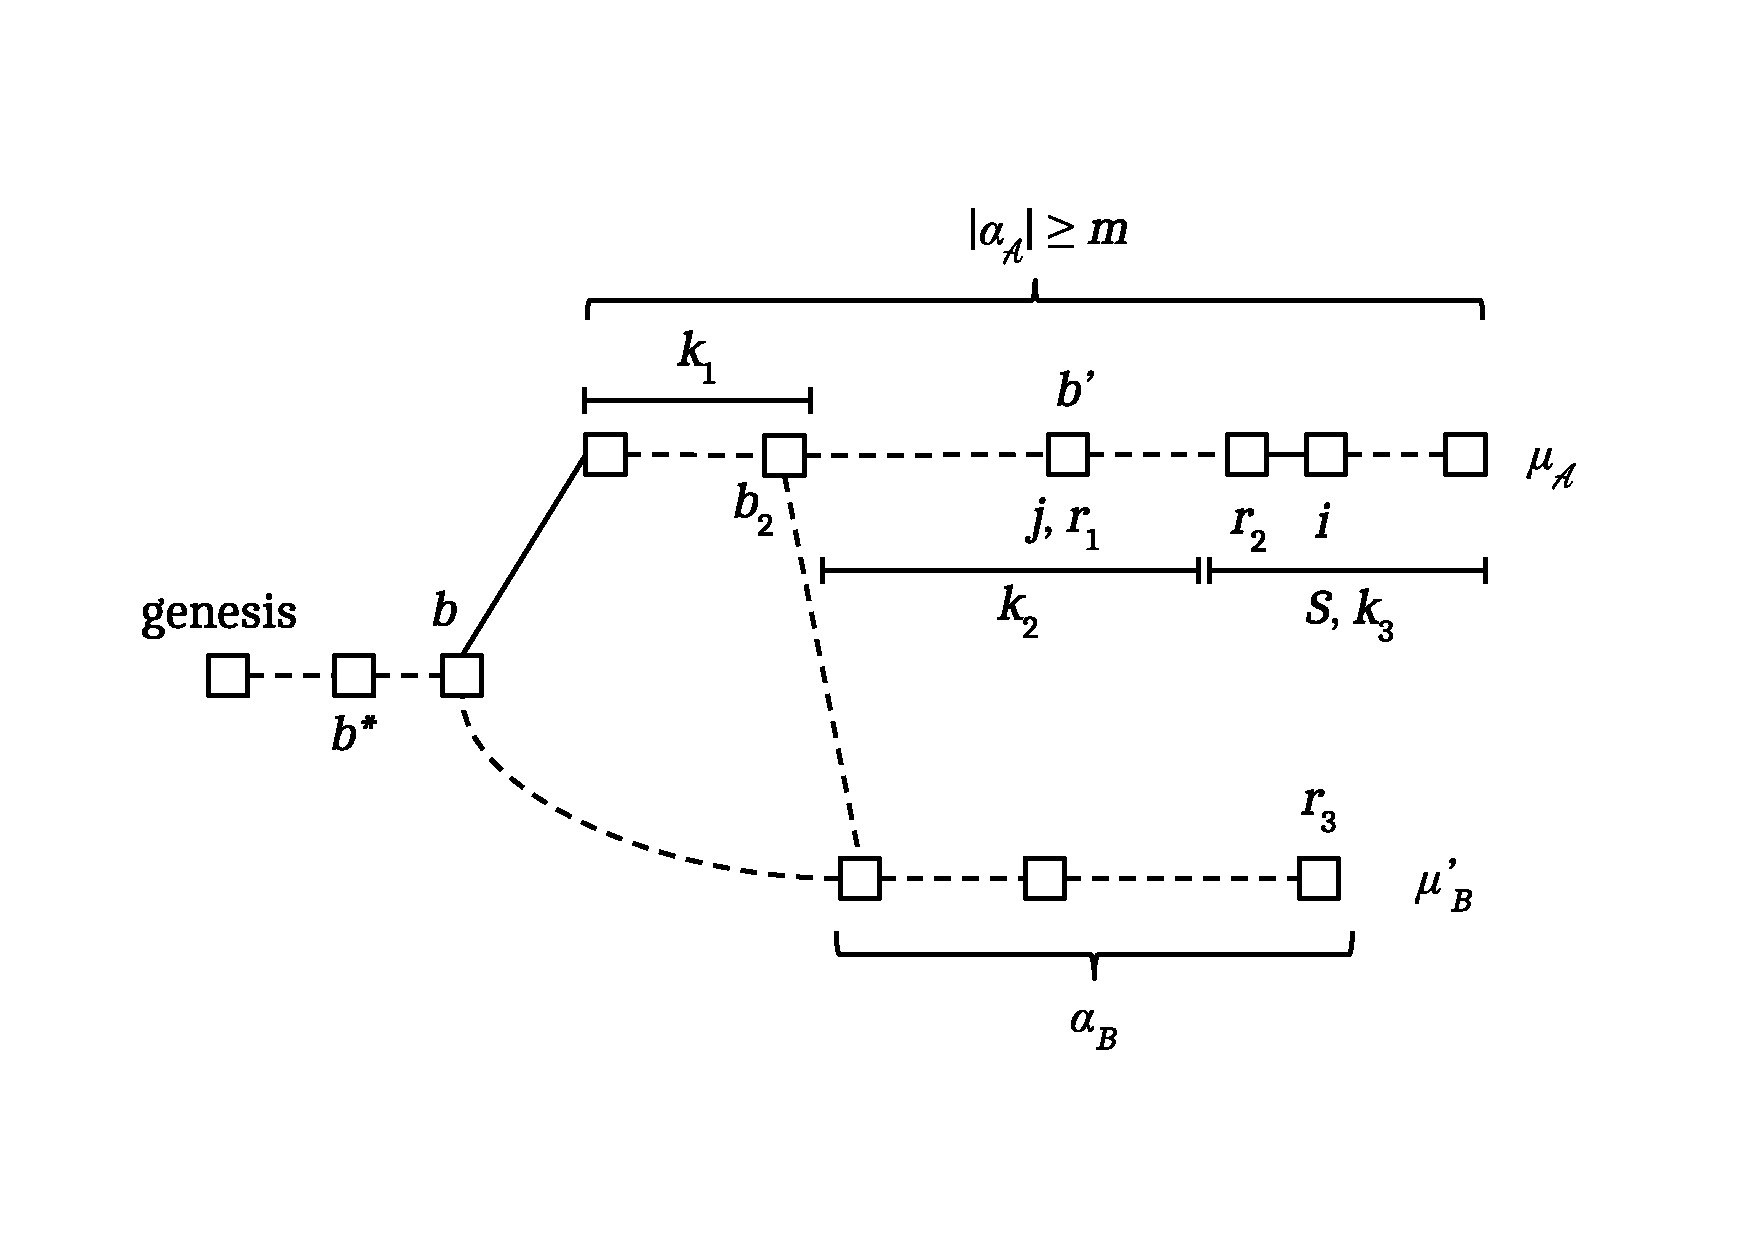
\includegraphics[width=0.8 \columnwidth,keepaspectratio]{figures/security-proof-chain.pdf}
        \label{fig.sec-comparison}
    \end{figure*}

    \textbf{Claim 1b: } If $\mu_\mathcal{A} < \mu_B'$ then
    $|\alpha_\mathcal{A}[1:] \cap \alpha_B\downchain[1:]| \leq 2^{\mu_B' - \mu_\mathcal{A}} k_1$.

    First, observe that, because the adversary is winning, therefore
    $|\alpha_\mathcal{A}| > 2^{\mu_B' - \mu_\mathcal{A}}m$.
    Suppose for contradiction that $|\alpha_\mathcal{A}[1:] \cap
    \alpha_B\downchain[1:]| > 2^{\mu_B' - \mu_\mathcal{A}} k_1$. This means
    there are indices $1 \leq i < j$ such that
    $|\chain_B\upchain^{\mu_\mathcal{A}}[i:j]| > 2^{\mu_B' - \mu_\mathcal{A}}
    k_1$ but
    $|\chain_B\upchain^{\mu_\mathcal{A}}[i:j]\downchain\upchain^{\mu_B'}| = 0$.
    But this contradicts the goodness of $\chain_B\upchain^{\mu_B'}$. Therefore
    there are more than $2^{\mu_B' - \mu_\mathcal{A}}(k_2 + k_3)$ blocks in
    $\alpha_\mathcal{A}$ that are not in $\alpha_B$, and clearly also more than $k_2 + k_3$ blocks.

    From Claim 1a and Claim 1b, we conclude that there are at least $k_2 + k_3$
    blocks after block $b$ in $\alpha_\mathcal{A}$ which do not exist in
    $\alpha_B$. We now set $b_2 = \textsf{LCA}(\chain_B, \alpha_\mathcal{A})$.

    \textbf{Claim 2: } At least $k_3$ superblocks of $\alpha_\mathcal{A}$ are
    adversarially generated.

    We show this by showing that $\alpha_\mathcal{A}[k_2 + 1:]$ contains
    no honestly mined blocks. By contradiction, assume that the block
    $\alpha_\mathcal{A}[i]$ for some $i \geq k_1 + k_2 + 1$ was honestly generated.
    This means that an honest party had adopted the chain
    $\alpha_\mathcal{A}[i - 1]$ at some round $r_2 \leq r_3$. Because of the
    way the honest parties adopt chains, the superchain
    $\alpha_\mathcal{A}[:i - 1]$ has an underlying properly constructed
    $0$-level anchored chain $\chain_\mathcal{A}$ such that
    $\chain_\mathcal{A} \subseteq \alpha_\mathcal{A}[:i - 1]$. Let $j$ be
    the index of block $b_2$ within $\chain_\mathcal{A}$.  As
    $\alpha_\mathcal{A} \subseteq \chain_\mathcal{A}$, observe that
    $|\chain_\mathcal{A}[j + 1:]| > i -
    1 \geq k_2 + k_1$. Therefore $\chain_\mathcal{A}[:-(k_2 + k_1)] \not\preccurlyeq
    \chain_B$. But $\chain_\mathcal{A}$ was adopted by an honest party at
    round $r_2$ which is prior to round $r_3$ during which $\chain_B$ was
    adopted by an honest party. This contradicts the Common Prefix
    \cite{backbone} property with parameter $k_2$.
    It follows that with overwhelming probability in $k_2$, the $k_3 = m - k_2 -
    k_1$ last blocks of the adversarial proof have been adversarially mined.

    \textbf{Claim 3: } $\mathcal{A}$ is able to produce a $\alpha_\mathcal{A}$
    that wins against $\alpha_B$ with negligible probability.

    Let $b'$ be the latest honestly generated block in $\alpha_\mathcal{A}$, or
    $b^*$ if no such block exists in $\alpha_\mathcal{A}$. Let $r_1$ be the
    round when $b^*$ was generated. Let $j$ be the index of $b^*$.
    Consider the set $S$ of consecutive rounds $r_1 \ldots r_3$. Every block
    in $\alpha_\mathcal{A}[-k_3:]$ has been adversarially generated during $S$
    and $|\alpha_\mathcal{A}[-k_3:]| = k_3$. $\chain_B$ is a chain adopted by an
    honest party at round $r_3$ and filtering the blocks by the rounds during
    which they were generated to obtain $\chain_B^S$, we see that $\chain_B^S =
    \chain_B\{b^*:\}$. But chain $\chain_B^S\upchain^{\mu_B'}$ is good with
    respect to $\chain_B^S$. Applying Lemma~\ref{lem.level-comparison}, we
    obtain that with overwhelming probability
    $2^{\mu_\mathcal{A}}|\alpha_\mathcal{A}\{b':\}| <
    \frac{1}{3}2^{\mu_B'}|\chain_B^S\upchain{\mu_B'}|$.

    But $|\alpha_B| \geq |\chain_B^S\upchain{\mu_B'}|$ and
    $|\alpha_\mathcal{A}\{b':\}| \geq |\alpha_\mathcal{A}| - k_2$, therefore
    $2^{\mu_\mathcal{A}}|\alpha_\mathcal{A}| - k_2 <
    \frac{1}{3}2^{\mu_B'}|\alpha_B|$.
    But $|\alpha_\mathcal{A}| - k_2 \geq k_3$, therefore
    $\frac{1}{3}2^{\mu_B'}|\alpha_B| > k_3$ and so $2^{\mu_B'}|\alpha_B| > 3k_3$
    Taking $k_2 = k_3$, we obtain
    $2^{\mu_\mathcal{A}}|\alpha_\mathcal{A}| <
    \frac{1}{3}3k_3 + k_3 = 2k_3 < 2^{\mu_B'}|\alpha_B|$.
    But this contradicts the fact that
    $\pi_\mathcal{A} \geq \pi_A$, and so the claim is proven.

    Therefore we have proven that $2^{\mu_B'}|\pi_B\upchain^{\mu_B'}| >
    2^{\mu_\mathcal{A}}|\pi_\mathcal{A}^{\mu_\mathcal{A}}|$.
    From the definition of $\mu_B$, we know that
    $2^{\mu_B}|\pi_B\upchain^{\mu_B}| \geq 2^{\mu_B'}|\pi_B\upchain^{\mu_B'}|$,
    and therefore we conclude that $2^{\mu_B}|\pi_B\upchain^{\mu_B}| >
    2^{\mu_\mathcal{A}}|\pi_\mathcal{A}\upchain^{\mu_\mathcal{A}}|$.
    \Qed
    % At the end of round $r_1$, $b'$ was diffused and hence all honest party
    % chains must all have adopted a chain of at least $c + j + 1$ superblocks of
    % level $\mu$.
%
    % Let $z$ be the number of $\mu$-level superblocks
    % generated by the adversary during those rounds, and observe that $z \geq m
    % - (j + 1) \geq k_3$.
    % From the assumption that the execution is typical, it
    % follows that either $Z^\mu(S) < k_3$, or that $Z^\mu(S)$ and $X^\mu(S)$
    % must be distributed close to their respective means. But in order for the
    % adversary to have generated $z$ blocks in $S$, it must hold that $Z^\mu(S)
    % \geq k_3$, and therefore $Z^\mu(S) < (1 - \frac{\delta}{2})X^\mu(S)$. However,
    % this means that the honest $\mu$-level superchain has grown by more than
    % $z$ superblocks and now contains at least $c + m$ superblocks. Therefore,
    % the honest chain now contains more than $c + j + 1 + z$ superblocks, while
    % the adversarial chain contains exactly $c + j + 1 + z$ superblocks.
    % $\textsf{maxChain}$ could not have returned true and
    % $\overline{\Pi}_\mathcal{A}$ could not have been the winning proof.
\end{proof}
